%% CIERA REU Template, using AASTeX v7+ (7.0.2, June 2026)
\documentclass[twocolumn]{aastex702}

%% You might consider other or additional options:
%\documentclass[linenumbers,amsmath]{aastex702}
%\documentclass[twocolumn,linenumbers,longauthor,trackchanges]{aastex702}
%% For all options, see https://journals.aas.org/aastexguide/#style_options

%% Define new commands here
\newcommand\latex{La\TeX}
\newcommand{\Msun}{$M_{\sun}$}
\newcommand{\Lsun}{$L_{\sun}$}
\newcommand{\solperyr}{$M_{\sun}$ yr$^{-1}$}
\newcommand{\solpermyr}{$M_{\sun}$ Myr$^{-1}$}
\newcommand{\solperpc}{$M_{\sun}$ pc$^{-2}$}
\newcommand{\SigGas}{$\Sigma_{\mathrm{gas}}$}
\newcommand{\SigSFR}{$\Sigma_{\mathrm{SFR}}$}

%% Optional: tells LaTeX to search for image files in the 
%% current directory as well as in the figures/ folder.
%\graphicspath{{./}{figures/}}

\begin{document}

\title{CIERA REU Template: Research Summary}

% Author Blocks: each author needs an \author, \affiliation, and \email entry
\author[orcid=0000-0001-6421-0953]{L. Clifton Johnson}
\affiliation{Center for Interdisciplinary Exploration and Research in Astrophysics (CIERA) and Department of Physics and Astronomy, Northwestern University, 1800 Sherman Ave., Evanston, IL 60201, USA}
\email{lcj@northwestern.edu}
\correspondingauthor{L. Clifton Johnson}

\author[orcid=0000-0002-3881-9332]{Aaron Geller}
\affiliation{Center for Interdisciplinary Exploration and Research in Astrophysics (CIERA) and Department of Physics and Astronomy, Northwestern University, 1800 Sherman Ave., Evanston, IL 60201, USA}
\affiliation{Research Computing and Data Services, Northwestern University Information Technology, 1800 Sherman Ave., Evanston, IL 60201, USA}
\email{a-geller@northwestern.edu}

\begin{abstract}

This template is meant as a starting point for CIERA REU cohort members for writing their research summary document. The template describes information about the Research Notes of the American Astronomical Society (RNAAS), as a model for the length and scope of your document. However, summary documents do not need to be submitted to RNAAS and therefore do not need to follow its strict format limits: one figure or table, abstract limit of 150 words, and text limit of 1500 words.

\end{abstract}

%% The AAS Journals now uses Unified Astronomy Thesaurus (UAT) concepts:
%% https://astrothesaurus.org
%% You can use the \uat command to link your UAT concepts back its source.
\keywords{\uat{Galaxies}{573} --- \uat{Cosmology}{343} --- \uat{High Energy astrophysics}{739} --- \uat{Interstellar medium}{847} --- \uat{Stellar astronomy}{1583} --- \uat{Solar physics}{1476}}

%% Start the main body of the article. If no sections in the 
%% research note leave the \section call blank to make the title.
\section{Introduction} 
\label{sec:intro}

This is paragraph demonstrates use of references and labels, as well as citations of references. Section \ref{sec:intro} and it contains Figure \ref{fig:1}.  \citet{Geller2019} says eccentricity is important.  Star clusters are great \citep{Geller2019}.

I also include a figure here to demonstrate that you can place a graphic in a specific location and make it equal to one column width, as shown in Figure \ref{fig:logo}.

\begin{figure}[h!]
    \centering
    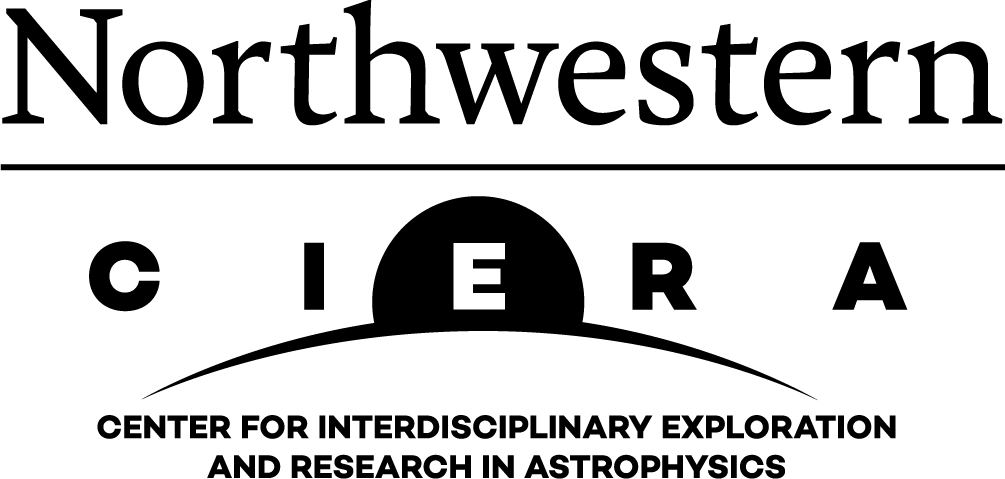
\includegraphics[width=0.8\linewidth]{figures/CIERA_formal_vert_black.png}
    \caption{A CIERA Logo. Other options for CIERA logos can be found here: \href{https://nuwildcat.sharepoint.com/:f:/s/RCH-ciera/EksTTlql9cBBiyAiR7aPa6YBo2Fw-Rexg2aCcZRLpJdY1A?e=TGDjqJ}{CIERA Logos}}
    \label{fig:logo}
\end{figure}

\section{\latex\ Examples}
\label{sec:tex}

For a rich example of AAS\TeX\ behavior, please see the \href{https://journals.aas.org/aastex-package-for-manuscript-preparation/#_download}{AAS\TeX\ full distribution download} which includes the \texttt{sample702.tex} example file. You can also access the Overleaf version of this CIERA REU template at \href{https://www.overleaf.com/read/pkqhhrpksvpd#a37b96}{this URL}.

\section{Research Notes}
\label{sec:rnaas}

\textit{Research Notes of the \href{https://aas.org}{American Astronomical Society}} (\href{http://rnaas.aas.org}{RNAAS}) is a publication in the AAS portfolio (alongside ApJ, AJ, ApJ Supplements, and ApJ Letters) through which authors can  promptly and briefly share materials of interest with the astronomical community in a form that will be searchable via ADS and permanently archived.

The astronomical community has long faced a challenge in disseminating information that may not meet the criteria for a traditional journal article. There have generally been few options available for sharing works in progress, comments and clarifications, null results, and timely reports of observations (such as the spectrum of a supernova), as well as results that wouldn’t traditionally merit a full paper (such as the discovery of a single exoplanet or contributions to the monitoring of variable sources). 

Launched in 2017, RNAAS was developed as a supported and long-term communication channel for results such as these that would otherwise be difficult to broadly disseminate to the professional community and persistently archive for future reference.

Submissions to RNAAS should be brief communications - 1,500 words or fewer \footnote{An easy way to count the number of words in a Research Note is to use the \texttt{texcount} utility installed with most \latex\ installations, e.g.,  \texttt{texcount -incbib -v3 rnaas.tex}). You can also use the overleaf ``Word Count'' utility under ``Menu'' in the upper left.  Another option is by copying the words into MS/Word, and using ``Word Count'' under the Tool tab.}, and no more than a single figure (e.g. Figure \ref{fig:1}) or table (but not both) - and should be written in a style similar to that of a traditional journal article, including references, where appropriate, but not including an abstract.

Unlike the other journals in the AAS portfolio, RNAAS publications are not peer reviewed; they are, however, reviewed by an editor for appropriateness and format before publication. If accepted, RNAAS submissions are typically published within 72 hours of manuscript receipt. Each RNAAS article is issued a DOI and indexed by ADS \citep{2000A&AS..143...41K} to create a long-term, citable record of work.

Articles can be submitted in \latex, MS/Word, or via the direct submission via the \href{http://www.overleaf.com}{Overleaf} online collaborative editor.

Authors are expected to follow the AAS's ethics \citep{2006ApJ...652..847K}, including guidance on plagiarism \citep{2012AAS...21920404V}.

%% An example figure call using figure* that spans the full page width
%% and \includegraphics with explicit scale
\begin{figure*}
\begin{center}
\includegraphics[scale=0.85,angle=0]{figures/aas.pdf}
\caption{Top page of the AAS Journals' website, \url{http://journals.aas.org},
on October 15, 2017.  Each RNAAS manuscript is only allowed one figure or table (but not both). Including the
\href{http://journals.aas.org//authors/data.html\#DbF}{data behind the figure}
in a Note is encouraged, and the data will be provided as a link in the
published Note.\label{fig:1}}
\end{center}
\end{figure*}

%% An example table using AASTeX's deluxetable. Note that since
%% only one figure OR one table is allowed this is commented out.
\begin{deluxetable}{ccl}
\tablecaption{Example table some English and Greek letters\label{tab:1}}
\tablehead{
\colhead{Index number} & \colhead{English} & \colhead{Greek}
}
\startdata
1 & a & alpha ($\alpha$) \\
2 & b & beta ($\beta$) \\
3 & c & gamma ($\gamma$) \\
4 & d & delta ($\delta$) \\
5 & e & epsilon ($\epsilon$) \\
\enddata
\tablecomments{Long tables should only show a short example with the full version as a machine readable table with the article.}
\end{deluxetable}  

\begin{acknowledgments}

This material is based upon work supported by the U.S. National Science Foundation under Award No. AST-2446392.

\end{acknowledgments}

\software{Astropy \citep{Astropy13, Astropy18, Astropy22}, Matplotlib \citep{Hunter07}}

\bibliographystyle{aasjournalv7.1}
\bibliography{references}

\end{document}
